\PassOptionsToPackage{unicode=true}{hyperref} % options for packages loaded elsewhere
\PassOptionsToPackage{hyphens}{url}
%
\documentclass[12pt,]{article}
\usepackage{lmodern}
\usepackage{amssymb,amsmath}
\usepackage{ifxetex,ifluatex}
\usepackage{fixltx2e} % provides \textsubscript
\ifnum 0\ifxetex 1\fi\ifluatex 1\fi=0 % if pdftex
  \usepackage[T1]{fontenc}
  \usepackage[utf8]{inputenc}
  \usepackage{textcomp} % provides euro and other symbols
\else % if luatex or xelatex
  \usepackage{unicode-math}
  \defaultfontfeatures{Ligatures=TeX,Scale=MatchLowercase}
\fi
% use upquote if available, for straight quotes in verbatim environments
\IfFileExists{upquote.sty}{\usepackage{upquote}}{}
% use microtype if available
\IfFileExists{microtype.sty}{%
\usepackage[]{microtype}
\UseMicrotypeSet[protrusion]{basicmath} % disable protrusion for tt fonts
}{}
\IfFileExists{parskip.sty}{%
\usepackage{parskip}
}{% else
\setlength{\parindent}{0pt}
\setlength{\parskip}{6pt plus 2pt minus 1pt}
}
\usepackage{hyperref}
\hypersetup{
            pdfborder={0 0 0},
            breaklinks=true}
\urlstyle{same}  % don't use monospace font for urls
\usepackage[margin=1in]{geometry}
\usepackage{longtable,booktabs}
% Fix footnotes in tables (requires footnote package)
\IfFileExists{footnote.sty}{\usepackage{footnote}\makesavenoteenv{longtable}}{}
\usepackage{graphicx,grffile}
\makeatletter
\def\maxwidth{\ifdim\Gin@nat@width>\linewidth\linewidth\else\Gin@nat@width\fi}
\def\maxheight{\ifdim\Gin@nat@height>\textheight\textheight\else\Gin@nat@height\fi}
\makeatother
% Scale images if necessary, so that they will not overflow the page
% margins by default, and it is still possible to overwrite the defaults
% using explicit options in \includegraphics[width, height, ...]{}
\setkeys{Gin}{width=\maxwidth,height=\maxheight,keepaspectratio}
\setlength{\emergencystretch}{3em}  % prevent overfull lines
\providecommand{\tightlist}{%
  \setlength{\itemsep}{0pt}\setlength{\parskip}{0pt}}
\setcounter{secnumdepth}{5}
% Redefines (sub)paragraphs to behave more like sections
\ifx\paragraph\undefined\else
\let\oldparagraph\paragraph
\renewcommand{\paragraph}[1]{\oldparagraph{#1}\mbox{}}
\fi
\ifx\subparagraph\undefined\else
\let\oldsubparagraph\subparagraph
\renewcommand{\subparagraph}[1]{\oldsubparagraph{#1}\mbox{}}
\fi

% set default figure placement to htbp
\makeatletter
\def\fps@figure{htbp}
\makeatother

\usepackage{graphicx}
\usepackage{wrapfig}
\usepackage[final]{pdfpages}
\usepackage{multicol}
\usepackage{amsfonts}
\usepackage{amssymb}
\usepackage{amsmath}
\usepackage{fancyhdr}
\usepackage{subcaption}
\usepackage{booktabs}
\usepackage[font=small]{caption}
\usepackage{float}
\usepackage{xcolor}
\usepackage{listings}
\usepackage{color}
\usepackage[titletoc,title,toc,page]{appendix}
\newcommand{\bmcols}{\begin{multicols}{2}}
\newcommand{\emcols}{\end{multicols}}
\usepackage{booktabs}
\usepackage{longtable}
\usepackage{array}
\usepackage{multirow}
\usepackage{wrapfig}
\usepackage{float}
\usepackage{colortbl}
\usepackage{pdflscape}
\usepackage{tabu}
\usepackage{threeparttable}
\usepackage{threeparttablex}
\usepackage[normalem]{ulem}
\usepackage{makecell}

\author{}
\date{\vspace{-2.5em}}

\begin{document}

\renewcommand{\appendixpagename}{\huge \selectfont Apêndice}
\renewcommand{\appendixname}{Apêndice}
\renewcommand{\appendixtocname}{Apêndice}

\setlength{\columnsep}{1cm}

\providecommand{\keywords}[1]{\def\and{{\textperiodcentered} }
\par\addvspace\baselineskip
\noindent\keywordname\enspace\ignorespaces #1}

\begin{center} 


{\bf \Large Predict responses to the marketing campaign with classification models}\\[0.5cm]
{\large Name: Suellen Sena da Silva} \\[1cm]      

\end{center}

\hypertarget{exploratory-analyses}{%
\section{Exploratory analyses}\label{exploratory-analyses}}

\quad Initially, it is important to observe the structure of the data
that will be used. The \(marketing\) \(training\) and \(marketing\)
\(test\) datasets have different types of variables: quantitative
(continuous) and qualitative (categorical and ordinal). It is
interesting to analyze the heterogeneous correlation matrix, that
computes Pearson correlations between numeric variables, polyserial
correlations between numeric and qualitative variables, and polychoric
correlations between qualitative variables. The matrix is represented in
the Figure \ref{fig:fig1}. From the correlation matrix it is possible to
create some hypotheses, as the correlation of the response variable
\(responded\) with the variables \(pmonths\), \(nr.employed\),
\(euribor3m\), \(emp.var.rate\), \(pdays\). In addition, it is noted
that the variables \(pdays\) and \(pmonths\) have a correlation equal to
1, which causes one of these two variables to be discarded from the
model to avoid multicollinearity.

\quad The training dataset has missing values for the variables
\(custAge\), \(schooling\) and \(days\) \(of\) \(week\). However,
\(custAge\) is a continuous variable, so it was decided to transform it
into a categorical variable to solve the problem with hot enconded. Ages
were categorized into 10-year age's groups.

\begin{lstlisting}[frame=single,framerule=0pt,framesep=8pt, basicstyle=\tiny]

# Import packages 

library(tidyverse)
library(caret)
library(polycor)
library(e1071)
library(kableExtra)

# Read the datasets and create partition between train (80%) and test (20%)

train = read_csv("marketing_training.csv")
test = read_csv("marketing_test.csv")
test <- test[,-1] 

trainIndex <- train %>% 
  createDataPartition(y = train$responded, 
                      p = 0.8, list=F, times = 1)

# Convert all character variables in factor and
# N/A values in strings to hot enconded 


train$day_of_week <- ifelse(is.na(train$day_of_week), 
                            "na", 
                            train$day_of_week)

train <- train %>% 
  mutate_if(is.character, as.factor)

train$schooling <- ifelse(is.na(train$schooling), 
                          "na", 
                          train$schooling)


# Transform responded feature to factor (yes = 1, no = 0)

train$responded <- ifelse(train$responded == "yes", 1, 0) 

# Heterogeneous correlation matrix
hetcor(train) %>% 
  as.matrix() %>% 
    ggcorrplot(lab = TRUE, type = "lower")

\end{lstlisting}

\begin{figure}[H]

{\centering 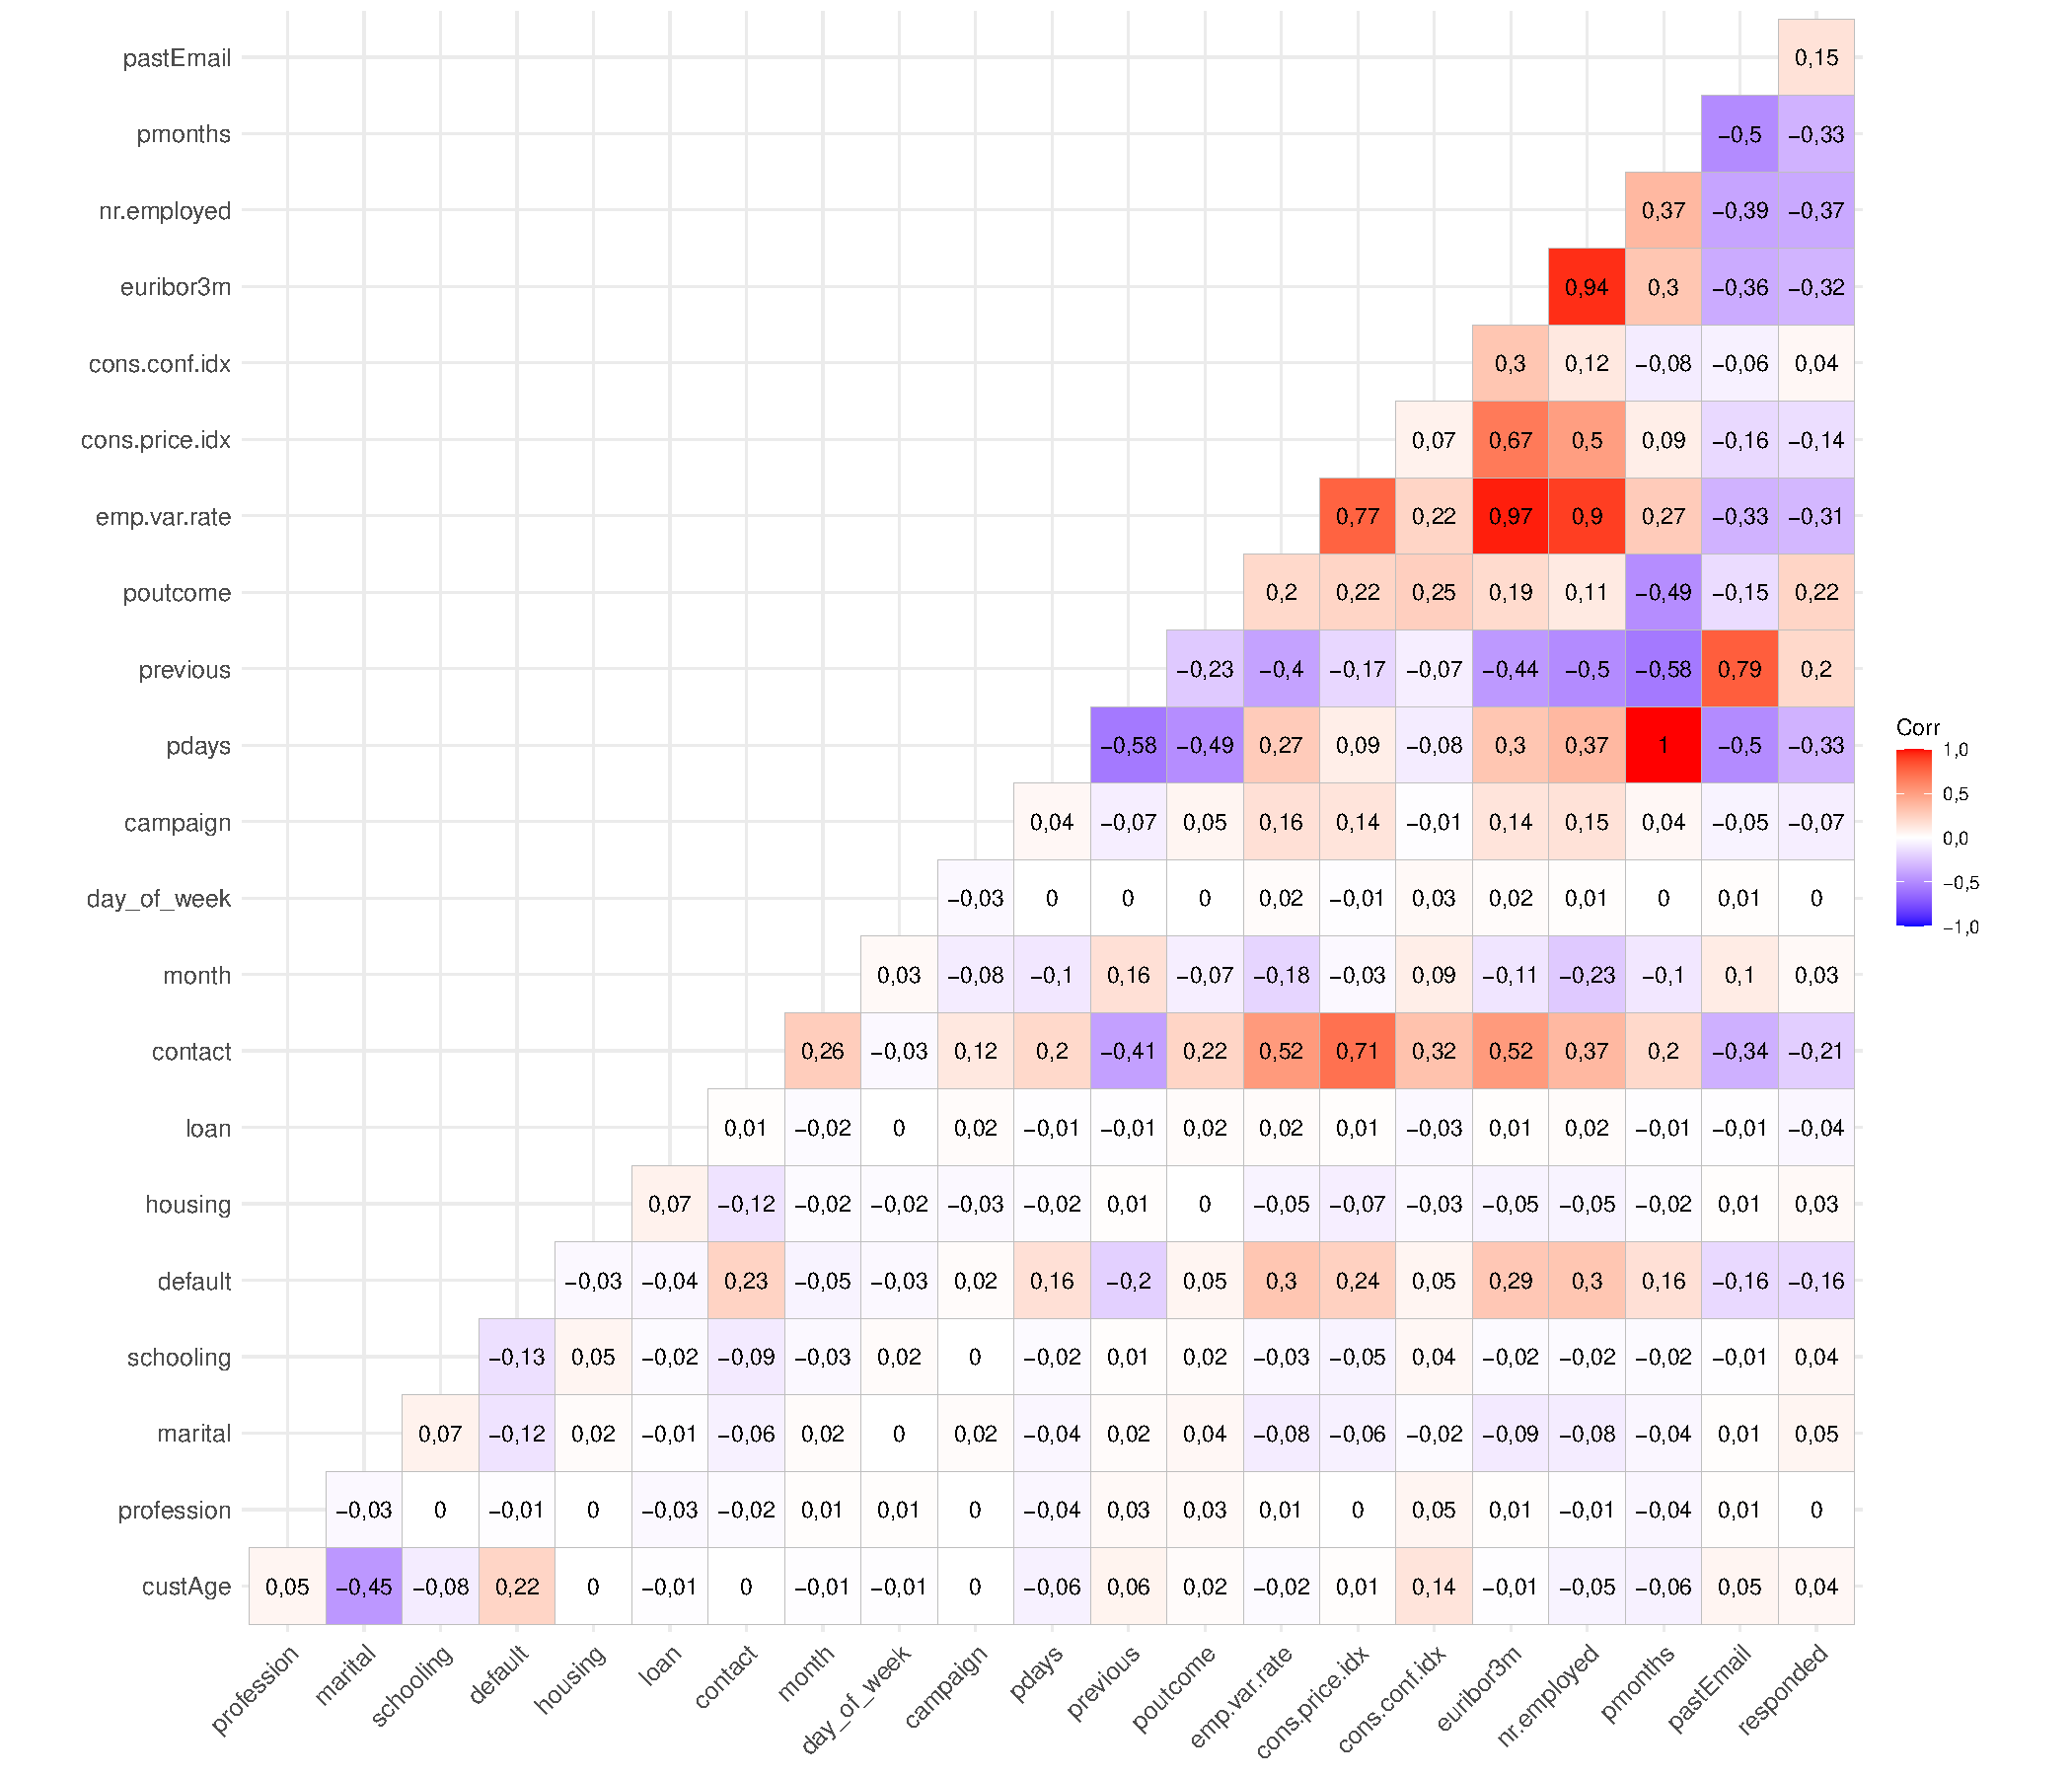
\includegraphics{cs_challenge_files/figure-latex/fig1-1} 

}

\caption{Heterogeneous correlation matrix.}\label{fig:fig1}
\end{figure}

\begin{lstlisting}[frame=single,framerule=0pt,framesep=8pt, basicstyle=\tiny]

# Hot encoded for factor variables

dummy <- dummyVars(" - .",  data=train)
train <- data.frame(predict(dummy, newdata = train)) 

train$responded <- train$responded %>% 
                      as.factor()

# Partition marketing_training.csv into train and test datasets

dftrain <- train[ trainIndex,]
dftest  <- train[-trainIndex,]


\end{lstlisting}

\hypertarget{pre-processing-and-classification-models}{%
\section{Pre processing and classification
models}\label{pre-processing-and-classification-models}}

\quad There are many different techniques that can improve the
performance of classification models. Then, the dataset was partitioned
randomly between training and testing, where each represents 80\% and
20\% of the data, respectively. Furthermore, it was considered the
technique \(cross-validation\) with \(number\) \(=\) \(5\). The
\(cross-validation\) method randomly divides the data into \(k\) blocks
of roughly equal size, each of the blocks is left out in turn and the
other \(k-1\) blocks are used to train the model. The held out block is
predicted and these predictions are summarized into some type of
performance measure (e.g.~accuracy or root mean squared error (RMSE)).
The \(k\) estimates of performance are averaged to get the overall
resampled estimate. It was also considered the use of the stepwise
method to select significant variables for the model, through the Akaike
Information Criterion (AIC). Finally, in classification problems, a
disparity in the frequencies of the observed classes can have a
significant negative impact on model fitting. One technique for
resolving such a class imbalance is to subsample the training data in a
manner that mitigates the issues. Examples of sampling methods for this
purpose are:

\begin{itemize}
   \item $down-sampling$: randomly subset all the classes in the training set so that their class frequencies match the least prevalent class;
   \item $up-sampling$: randomly sample (with replacement) the minority class to be the same size as the majority class.
\end{itemize}

\quad Different classification models were considered for this problem,
these are:

\begin{itemize}
   \item $Logistic$ $regression$: is the appropriate regression analysis to conduct when the dependent variable is dichotomous (binary).  Like all regression analyses, the logistic regression is a predictive analysis.  Logistic regression is used to describe data and to explain the relationship between one dependent binary variable and one or more nominal, ordinal, interval or ratio-level independent variables.;
   
   \item $K-nearest$ $neighbors$ $algorithm$: data classification algorithm that attempts to determine what group a data point is in by looking at the data points around it.An algorithm, looking at one point on a grid, trying to determine if a point is in group A or B, looks at the states of the points that are near it. The range is arbitrarily determined, but the point is to take a sample of the data. If the majority of the points are in group A, then it is likely that the data point in question will be A rather than B, and vice versa;
   
   \item  $Decision$ $tree$: builds classification or regression models in the form of a tree structure. It breaks down a dataset into smaller and smaller subsets while at the same time an associated decision tree is incrementally developed. The final result is a tree with decision nodes and leaf nodes;
    \item  $Random$ $Forest$: are an ensemble learning method for classification, regression and other tasks that operate by constructing a multitude of decision trees at training time and outputting the class that is the mode of the classes (classification) or mean/average prediction (regression) of the individual trees;
    \item  $Support$ $Vetor$ $Machine$: particular linear classifiers which are based on the margin maximization principle. They perform structural risk minimization, which improves the complexity of the classifier with the aim of achieving excellent generalization performance. The SVM accomplishes the classification task by constructing, in a higher dimensional space, the hyperplane that optimally separates the data into two categories.
\end{itemize}

\begin{lstlisting}[frame=single,framerule=0pt,framesep=8pt, basicstyle=\tiny]

# Logistic regression with stepwise features selection 

trainctrl <- trainControl(method = "cv", number = 5)

set.seed(42)
logstep.model = train(
  form = responded - .,
  data = dftrain,
  trControl = trainctrl,
  method = "glmStepAIC",
  family = "binomial", 
  metric="AIC"
)


# Logistic regression with up-sampling method for unbalanced data

trainctrl <- trainControl(method = "cv", number = 5, sampling="up")

set.seed(42)
logup.model = train(
  form = responded - .,
  data = dftrainup,
  trControl = trainctrl,
  method = "glm",
  family = "binomial", 
  metric="Accuracy"
)

# Logistic regression with down-sampling method for unbalanced data

trainctrl <- trainControl(method = "cv", number = 5, sampling="down")

set.seed(42)
logdown.model = train(
  form = responded - .,
  data = dftraindown,
  trControl = trainctrl,
  method = "glm",
  family = "binomial", 
  metric="Accuracy"
)


# Logistic regression

set.seed(42)
trainctrl <- trainControl(method = "cv", number = 5)

log.model = train(
  form = responded - .,
  data = dftrain,
  trControl = trainctrl,
  method = "glm",
  family = "binomial", 
  metric="Accuracy"
)


# K-nearest neighbors algorithm with up-sampling method and centering features

trainctrl <- trainControl(method = "cv", number = 5, sampling="up")

set.seed(42)
knn.model <- train(responded, data=dftrainup, method = "knn",
                   tuneLength = 5,
                   trControl = trainctrl,
                   metric="Accuracy", 
                   preProcess = ("center"))


# Decision tree with up-sampling method

set.seed(42)
dt.model <- train(responded, data=dftrain, method = "rpart", 
                  tuneLength = 5,
                  trControl = trainctrl,
                  metric="Accuracy")


# Random forest with up-sampling method

set.seed(42)
rf.model <- train(responded, data=dftrainup, method = "rf", 
                  tuneLength = 5,
                  ntree = 10,
                  trControl = trainctrl,
                  metric="Accuracy")



# Support vector machine with up-sampling method

set.seed(42)
svm.model <- train(responded, data=dftrain, method = "svmRadial", 
                   tuneLength = 5,
                   trControl = trainctrl,
                   metric="Accuracy",
                   preProcess = ("center"))


svm.model = svm(formula = responded - .,
                 data = dftrainup,
                 type = 'C-classification',
                 kernel = 'linear')


# Logistic regression with up-sampling and stepwise method

trainctrl <- trainControl(method = "cv", number = 5, sampling="up")

set.seed(42)
logstepup.model = train(
  form = responded - .,
  data = dftrain,
  trControl = trainctrl,
  method = "glmStepAIC",
  family = "binomial", 
  metric="AIC"
)

\end{lstlisting}

\begin{table}[H]
\caption{\label{tab:}Accuracy and recall metrics.}
\centering
\fontsize{11}{13}\selectfont
\begin{tabular}[t]{llllllll}
\toprule
 Model & Accuracy & Recall (positive 0) & Recall (positive 1)  \\
 \midrule
Logistic up-sampling and stepwise & 0,80 & 0,85 & 0,67 &  \\
Logistic stepwise & 0,90 & 0,98 & 0,24 &  \\
Logistic up-sampling & 0,80  &  0,85 & 0,67 &  \\
Logistic down-sampling & 0,78 & 0,83 & 0,66 & \\
Logistic & 0,90 & 0,98  & 0,26 &  \\
KNN up-sampling & 0,69 & 0,85  & 0,69 &  \\
Decision tree up-sampling & 0,79 & 0.85 & 0,69 &  \\
Random forest up-sampling & 0,87 & 0,95 & 0,40 &  \\
SVM up-sampling & 0,82 & 0,88 & 0,49 &  \\
\bottomrule
\end{tabular}
\end{table}

\hypertarget{predictions-in-test-dataset}{%
\section{Predictions in test
dataset}\label{predictions-in-test-dataset}}

\quad The model was chosen based on the highest accuracy value and
recall for a category ``1 (yes)'', which represents a minority response.
The models fits in logistic regression and decision tree are superior
efficient then the others, however, the accuracy is greater in logistics
and it is not significantly lower on \(yes\) decision tree model's
category , that's why logistic regression was the chosen one to obtain
the test of dataset.

\begin{table}[H]

\caption{\label{tab:unnamed-chunk-8}Prediction in test dataset.}
\centering
\fontsize{11}{13}\selectfont
\begin{tabular}[t]{lr}
\toprule
Class & Predict\\
\midrule
0 & 1212\\
1 & 270\\
\bottomrule
\end{tabular}
\end{table}

\end{document}
